\documentclass[modern]{aastex61}
\usepackage{xspace}
\usepackage[utf8]{inputenc}
\usepackage[T1]{fontenc}
\usepackage{ulem}
\newcommand{\escapecmd}[1]{\texttt{\detokenize{#1}}}

% To allow putting figures in a subdir
\graphicspath{{figures/}}

\submitjournal{ApJ}

\shorttitle{Astropy Project II}
\shortauthors{Astropy Project et al.}

% Packages / projects / programming - for consistency!
\newcommand{\package}[1]{\texttt{#1}\xspace}
\newcommand{\github}{\package{GitHub}}
\newcommand{\python}{\package{Python}}
\newcommand{\astropy}{Astropy\xspace}
\newcommand{\astropypkg}{\package{astropy}}

% For consistency:
\newcommand{\sectionname}{Section\xspace}
\renewcommand{\figurename}{Figure\xspace}
\newcommand{\equationname}{Equation\xspace}
\renewcommand{\tablename}{Table\xspace}

% Words that should not be hyphenated
\hyphenation{NumFOCUS}

% For commenting - can be deleted before submission
\usepackage[colorinlistoftodos]{todonotes}
\newcommand{\inlinecomment}[2]{\todo[inline]{#1: #2}\xspace}
\newcommand{\comment}[2]{\todo{#1: #2}\xspace}

\begin{document}

\draft{\today}

\title{The Astropy Project}

\correspondingauthor{Astropy Coordination Committee}
\email{coordinators@astropy.org}

\author{Astropy Collaboration}

\begin{abstract}
% I (Adrian) took a first stab at the abstract, but it needs some work. Feel
% free to modify!
The \astropy project supports and fosters the development of open-source and openly-developed
\python packages that provide commonly-needed functionality to the astronomical
community.
A key element of the \astropy project is the core package \astropypkg, which serves as the
foundation for more specialized projects and packages.
In this article, we provide an overview of the organization of the \astropy
project and summarize key features in the core package as of the recent major
release, version 2.0.
We then describe the project infrastructure designed to facilitate and support
development for a broader ecosystem of inter-operable packages.
We conclude with a future outlook of planned new features and directions for the
broader \astropy project.
\end{abstract}

% Adrian PW: how are there still no software keywords in AAS journals?!?
\keywords{%
    Astrophysics - Instrumentation and Methods for Astrophysics
    ---
    methods: data analysis
    ---
    methods: miscellaneous
}


\section{Introduction} \label{sec:intro}
% first draft by Moritz (hamogu)
% heavily edited by Adrian PW - let me know if you want to revert anything!
All astronomical research makes use of software in some way.  Astronomy as a field has thus long supported the development of software tools
for astronomical tasks: from scripts that enable individual scientific research to software packages for small collaborations to data reduction pipelines for survey operations.
Some software packages are or were supported by large institutions and are intended for a wide range of users. These packages typically provide some level of documentation and user support or
training.
Other packages are developed by individual researchers or research groups and
are then typically used by smaller groups for more domain-specific purposes.
Whether for a package meant for wide distribution or for scripts and programs
for a specific research project, the implementation of astronomical software can
be eased through the use of a library that provides core functionality that is
common to many astronomical tasks.
The users of such software then also benefit from a community and ecosystem
built around a common foundation.
The \astropy project has grown to become this community for \python astronomy
software, and the \astropypkg core package a feature-rich \python library.

%\inlinecomment{Tom R}{the 'this community' above is a bit too general - do we mean it is the only community in astronomy, or in the Python astronomy world? I'd change this to either 'to become this community for Python astronomy software' or 'to become such a community'. For instance yt had a community before we came along for the simulation community, so I want to make sure we don't claim we are the only community out there.}
%\inlinecomment{Perry G}{Agreed}

The development of the \astropypkg core package began as a largely
community-driven effort to standardize core functionality for astronomical
software in \python.
In this way, its genesis differs from but builds upon many substantial and
% * <bsipocz@gmail.com> 2017-11-13T13:13:08.884Z:
%
% how do astroy builds upon these? or it's more like builds upon the developer experience?
%
%
% ^.
former astronomical software development efforts that were commissioned or
initiated through large institutional support, for example IRAF \citep[developed
at NOAO;][]{IRAF}, MIDAS \citep[developed at ESO;][]{MIDAS}, or Starlink
\citep[originally developed by a consortium of UK institutions and now
maintained by the East Asian Observatory;][]{starlink1982,starlink2013}.
More recently, community-driven efforts have seen significant success in the astronomical sciences \citep{yt}.

\python\footnote{\url{https://www.python.org/}} is an increasingly popular, general-purpose
programming language that is available under a permissive open source software license free of
charge for all major operating systems. The programming language has become especially popular
in the quantitative sciences, where researchers must simultaneously produce research, perform
data analysis, and develop software. A large part of this success owes itself to the vibrant
community of developers and a continuously-growing ecosystem of tools, web services, and stable
well-developed packages that enable easier collaboration on software development, easier
writing and sharing of software documentation, and continuous testing and validation of
software. While the programming language provides support for array representation and
arithmetic \citep[\package{numpy};][]{numpy}, a wide variety of functions for scientific
computing \citep[\package{scipy};][]{scipy}, and publication-quality plotting
\citep[\package{matplotlib};][]{matplotlib}, tens of thousands of other high-quality and easy-to-use
packages are available, which can help with tasks that are not astronomy specific but
might be performed in the course of astronomical research; e.g., interfacing with
databases or statistical inferences. More recently, the development of package managers such as
Anaconda\footnote{\url{https://anaconda.org/}} have streamlined the installation process for
most packages, significantly reducing the entry barrier for using many such libraries.

The \astropy project aims to provide an open-source and open-development core
package (\astropypkg) and an ecosystem of \emph{affiliated packages} that
support astronomical functionality in the \python programming language.
The \astropypkg core package is now a feature-rich library of sufficiently
general tools and classes that supports the development of more specialized
code. An example of such functionality is reading and writing FITS files: It would be
time consuming and impractical for multiple groups to implement the FITS
standard \citep{FITS} and maintain software for such a general-purpose need.
Another example of such a common task is in dealing with representations of and
transformations between astronomical coordinate systems.

The \astropy project aims to develop and provide high-quality code and
documentation according to the best practices in software development.
The project makes use of these tools to do so without central institutional
oversight.
The first public release of the \astropypkg package is described in
\cite{astropy}. Since then, the \astropypkg package has been
used in hundreds of projects and the scope of the package has grown
considerably. At the same time, the scientific community
contributing to the project has grown tremendously and an ecosystem
of packages supporting or affiliated with the \astropypkg core has
developed.
In this paper, we describe the current status of the \astropy community and the
\astropypkg core package and discuss goals for future development.

We start by describing the way the \astropy project functions and is organized
in \sectionname~\ref{sec:org}. We then describe the main software efforts
developed by the \astropy project itself: a core package called \astropypkg
(\sectionname~\ref{sec:core}) and several separate packages that help maintain
the infrastructure for, e.g., testing and documentation
(\sectionname~\ref{sec:infrastructure}). We end with a short vision for
the future of \astropy in particular and astronomical software in general
in \sectionname~\ref{sec:future}.

\section{Organization and infrastructure}
\label{sec:org}

\subsection{Coordination of Astropy}
% draft by ?? (BMS thinks Erik)
% edited by Adrian PW
\label{sect:coordcom}
From its inception, \astropy has required coordination to ensure the project
as a whole and its coding efforts are consistent and reasonably efficient.
While many \python projects adopt a ``Benevolent Dictator For Life'' (BDFL)
model, \astropy has instead opted for a \emph{coordination committee}.  This
is in part due to the nature of the project as a large-scale collaboration
between many contributors with many interests, and in part due to simply the
amount of work that needs to get done.  For the latter reason, the
project has expanded the committee from three to four members starting in
2016.

For resolving disagreements about the \astropypkg core package or other \astropy-managed code, the coordination committee primarily acts to work toward consensus, or when consensus is difficult to achieve, generally acts as a ``tie-breaker.''
The committee also oversees affiliated package applications to ensure they are in keeping with \astropy's vision and philosophy, as well as the associated procedures.
Additionally, the committee oversees the assignment of roles (primarily driven by already-existing contributions), and increasingly has acted as the ``face'' of the Project, providing contact with organizations like NumFOCUS (the body that holds any potential funding in trust for \astropy) or the American Astronomical Society (AAS).

\subsection{Astropy development model}
% draft by Adrian PW and Erik T.
Code is contributed to the \astropypkg core package or modified through ``pull
requests'' (via \github) that often contain several \texttt{git} commits.
Pull requests may fix bugs, implement new features, or improve or modify the
infrastructure that supports the development and maintenance of the package.
Individual pull requests are generally limited to a single conceptual addition
or modification to make code review tractable.
Pull requests that modify or add code to a specific subpackage must be reviewed
and approved by one of the subpackage maintainers before it is merged into the
core codebase.
Bugs and feature requests are reported via the \github issue tracker and labeled
with a set of possible labels that help classify and organize the issues.
The development workflow is detailed in the \astropypkg
documentation.\footnote{\emph{How to make a code contribution},
\url{http://docs.astropy.org/en/latest/development/workflow/development_workflow.html}}

\begin{figure}
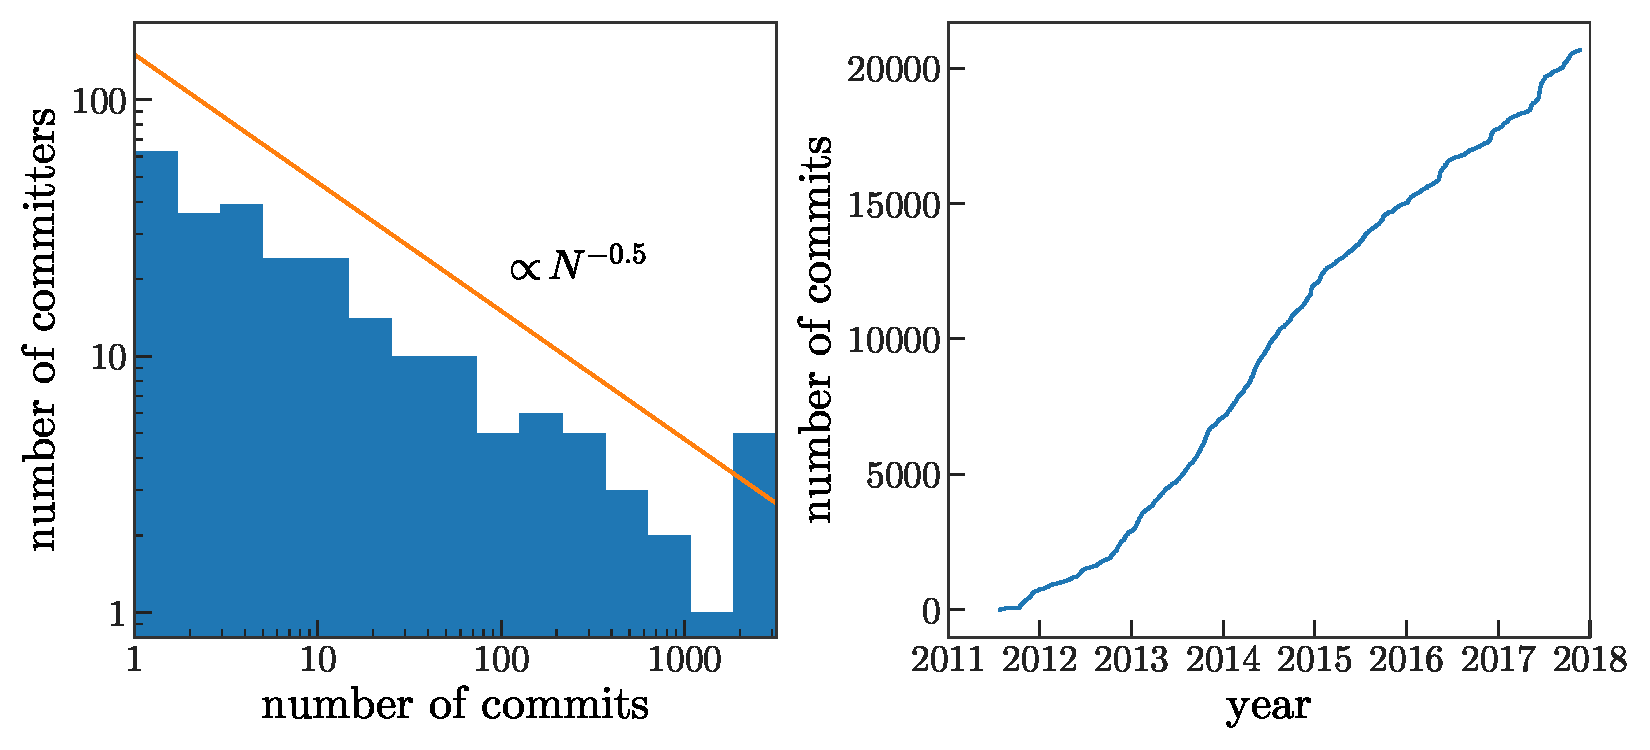
\includegraphics[width=\textwidth]{ncommits.pdf}
\caption{%
    \emph{Left panel}: Distribution of number of commits per committer.
    \emph{Right panel}: Cumulative number of commits to the \astropypkg core
    package over time.
    \label{fig:ncommits}
}
\end{figure}

As of version 2.0, \astropypkg contains $212244$ lines of code\footnote{This
line count includes comments, as these are often as important for
maintainability as the code itself.  Without comments there are $142197$ lines
of code.} contributed by $232$ unique contributors over $19270$ \texttt{git}
commits.
\figurename~\ref{fig:ncommits}, left, shows the distribution of total number of
commits per contributor as of November 2017.
The relative flatness of this distribution (as demonstrated by its log-log slope of
$-0.5$) shows that the \astropypkg core package has been developed by a broad
contributor base.  A leading group of 6 developers have each added over 1000
commits to the repository, and $\sim 20$ more core contributors with at least
100 commits.
However, the distribution of contribution level (number of commits) continues
from 100 down to a single commit.
In this sense, the development of the core package has been a true community
effort and is not dominated by a single individual.
It is also important to note that the number of commits is only a rough metric
of contribution, as a single commit could be a critical fix in the package or a
fix for a typographical error.
\figurename~\ref{fig:ncommits}, right, shows the number of commits as a
function of time since the genesis of the \astropypkg core package.
The package is still healthy: new commits are and have been contributed at a
steady rate throughout its existence.

\subsection{APEs - Astropy Proposals for Enhancement}
% draft by hamogu
% edited by Adrian PW

Central to the success of \astropy is an open environment where anybody can
contribute to the project.
This model leads to an ``organic'' growth, where different features are
implemented by different people with different programming styles and
interfaces.
Thus, \astropy has a mechanism to more formally propose significant changes to
the core package (e.g., re-writing the coordinates subpackage; \citealt{ape5}),
to plan out major new features (e.g., a new file format; \citealt{ape6}), or
institute new organization-wide policies (e.g., adopting a code of conduct;
\citealt{ape8}).
This mechanism is called ``Astropy Proposal for Enhancement'' (APE) and are
modeled after the ``Python Enhancement Proposals'' (PEP) that guide the
development of the \python programming language.
In an APE, one or more authors describe in detail the proposed changes or
additions, including a rationale for the changes, how these changes will be
implemented, and in the case of code, what the interface will be \citep{ape1}.
The APEs are discussed and refined by the community before much work is invested
into a detailed implementation; anyone is welcome to contribute to these
discussions during the open consideration period. APEs are proposed via pull
requests on a dedicated GitHub repository\footnote{\url{https://github.com/astropy/astropy-APEs}};
anyone can therefore read the proposed APEs and leave in-line comments.
When a community consensus emerge, the APEs are accepted and become
the basis for future work.
In cases where consensus cannot be reached, the
\astropy coordination committee may decide to close the discussion and
make an executive decision based on the community input on the APE in question.


\subsection{Concept of affiliated packages}
% it may be described in previous subsection, if not the Brigitta can try to
% write it up
% edited by Adrian PW

A major part of the \astropy project is the concept of
``Affiliated Packages''. An affiliated package is an astronomy-related
\python package that is not part of the \astropypkg core package, but
has requested to be included as part of the \astropy project's
community. These packages support the goals and vision of \astropy of
improving code re-use, interoperability, and embracing good coding
practices such as testing and thorough documentation.

Affiliated packages contain functionality that is more specialized,
have license incompatibilities, or have external dependencies (e.g., GUI
libraries) that make these packages more suitable to be separate from the
\astropypkg core package.
Affiliated packages may also be used to develop substantial new functionality
that will eventually be incorporated into the \astropypkg core package
(e.g., \texttt{wcsaxes}).
New functionality benefits from having a rapid development and release cycle that is not tied to that of the \astropypkg core (\sectionname~\ref{sect:releasecycle}).
% AG: rephrased this.
%Initially separate packages with typically rapid initial development and new experimental features benefit from having a release cycle that is not tied to the

Affiliated packages are listed on the main \astropy website and advertised to the community through \astropy mailing lists. Therefore, becoming an affiliated package is a good way for new and existing packages to gain exposure while promoting \astropy's high standard for code and documentation quality. This process of listing and promoting affiliated packages is one way in which the \astropy project tries to increase code re-use in the astronomical community.

Packages can become affiliated to \astropy by applying for this status on a public mailing list. The coordination committee (\sectionname~\ref{sect:coordcom}) reviews such requests and issues recommendations for the improvement of a package, where applicable.

%\subsection{Accuracy testing across many different implementation}

\subsection{Release cycle and Long Term Support}
\label{sect:releasecycle}
% This could also include information about the development cycle
% Brigitta can writes this up if there's no other taker
% edited by Adrian PW

The \astropypkg package has a regular release schedule consisting of new significant
releases every 6 months, with bugfix releases as needed \citep{ape2}.
The major releases contain new features or any significant changes, whereas
the bugfix releases only contain fixes to code or documentation but no new
features.
Some versions are additionally designated as ``Long-term support'' (LTS)
releases, which continue to receive bug fixes for 2 years following the release
with no changes to the API\@.
The LTS versions are ideal for pipelines and other applications, where API
stability is essential.
The latest LTS release (v2.0) is also the last one that supports \python 2; It
will receive bug fixes until the end of 2019 \citep{ape10}.

The version numbering of the \astropypkg core package reflects this release
scheme: the core package version number uses the form \texttt{x.y.z}, where ``x'' is
advanced for LTS releases, ``y'' for non-LTS feature releases, and
``z'' for bugfix releases.

The released versions of the \astropypkg core package are available from several
of the \python distributions for scientific computing (e.g.,
\href{http://anaconda.org}{Anaconda}) and from the \python Package Index
(PyPI).\footnote{See the installation documentation for more information:
\url{http://docs.astropy.org/en/stable/install.html}}
Effort has been made to make \astropypkg available and easily installable across
all platforms; the package is constantly tested on different platforms as part
of our suite of continuous integration tests.

\subsection{Support of Astropy}

The \astropy project, as of the v2.0 release, does not receive any direct financial support for
the development of \astropypkg.  Development of the software, all supporting materials, and community support is provided
by individuals who work on the \astropy project in their own personal
time, by individuals or groups contributing to \astropy as
part of a research project, or contributions from institutions that allocate
people to work on \astropy.
A list of organizations that have contributed to \astropy in this manner
can be found in the Acknowledgements.

Different funding models have been proposed for support of \astropy
(e.g., \citealt{2016arXiv161003159M}), but a long-term plan
for sustainability has not yet been established.
The \astropy project has the ability to accept financial contributions
from institutions or individuals through the NumFOCUS\footnote{NumFOCUS
is a 501(c)(3) nonprofit that supports and promotes world-class, innovative,
open source scientific computing.} organization. NumFOCUS has to date covered the direct costs incurred by the \astropy project.

% Removing unless this gets written about in
% a later version
% This section should be a straight forward/factual description of the current
% funding and support provided to astropy with the purpose of explaining the
% current structure to the community


%\subsection{Difficulty of reversing design choices}
%Deciding if a feature should be included
%difficulty to decide where general use ends and "handy feature for some" starts, i.e. how to reject PRs or deal with maintenance burden

\section{Astropy Core Package v2.0}
\label{sec:core}
% Adrian
The \astropy project aims to provide \python-based packages for all tasks that
are commonly needed in a large subset of the astronomical community.
At the foundation is the \astropypkg core package, which provides general
functionality (e.g., coordinate transformations, reading and writing astronomical
files) or base classes for other
packages to utilize for a common interface (e.g., \texttt{NDData}).
In this section, we highlight new features introduced or substantially improved
since version v0.2 (previously described in \citealt{astropy}).  The \astropypkg
provides a full log of changes\footnote{\url{https://github.com/astropy/astropy/blob/stable/CHANGES.rst}}
over the course of the entire project and more details about individual
subpackages are available in the documentation.\footnote{\url{http://docs.astropy.org/en/stable/}}
Beyond what is mentioned below, most subpackages have seen increased performance
since the release of the v0.2 package.


% \subsection{Analytic Functions}
% moved to models and depreciated --
% just here for completeness at the moment
%\inlinecomment{BMS}{I suggest to order the subsection lexicographically as reading the draft the current order seemed very random (unlike at the docs page where they the grouping logic is obvious)}
%\inlinecomment{Tom R}{the only issue is if we rely on having e.g. units described first if they are used later}

\subsection{Units}\label{sec:units}
% Adrian

The \texttt{astropy.units} subpackage adds support for representing units and
numbers with associated units --- ``quantities'' --- in code.
Historically, quantities in code have often been represented simply as numbers,
with units implied or noted via comments in the code because of considerations
about speed: having units associated with numbers inherently adds overhead to
numerical operations.
In \texttt{astropy.units}, \texttt{Quantity} objects extend \texttt{numpy}
array objects and have been designed with speed in mind.

%\inlinecomment{Perry G}{Agreeing with Tom below, I would avoid using terms like subclass, decorators, mixin, namespace, (and perhaps even class, instead using objects consistently; this is no place to be pendantic about the distinction between classes and objects; even to the extent of adding a qualifying sentence somewhere like: "In this paper we will use object when we mean object or classes; in software there are important distinctions between the two terms, but they are not relevant in this paper."), and the like and replace them with more generic descriptions, e.g., "extended", or "tools to make defining functions that can use quantities simple to write" }
%\inlinecomment{Tom R}{I think saying 'subclass' here is too detailed and is mentioned below in 3.1.1 if needed - 'make it possible to attach units to numpy arrays' or something like that?}

As of \astropypkg version 2.0, units and quantities are prevalent in most other
\astropypkg subpackages and are thus a key concept for using the package as a
whole.
Units are intimately entwined in the definition of astronomical coordinates and
thus nearly all functionality in the \texttt{astropy.coordinates} subpackage
(see \sectionname~\ref{sec:coordinates}) depends on this functionality.
For most other subpackages, quantities are at least accepted, and often expected
by default.

The motivation and key concepts behind this subpackage were described in detail
in the previous paper \citep{astropy}, and thus here we primarily highlight new
features and improvements.

\subsubsection{Interaction with \package{numpy} arrays}

\texttt{Quantity} objects extend
\texttt{numpy.ndarray} objects and therefore
work well with many of the functions in \texttt{numpy} that support
array operations. For example, \texttt{Quantity} objects with angular
units can be directly passed in to the trigonometric functions implemented in
\texttt{numpy}. The units are internally converted to radians (what the \texttt{numpy}
trigonometric functions expect) before being passed to \texttt{numpy}.

%\subsubsection{Speed improvements}

%\inlinecomment{Tom R}{I wonder if we might just want to mention at the top level that performance has been improved in places? This seems a bit too detailed}

%The \texttt{Quantity} object is now significantly
        %faster than in early versions of \astropypkg. This is in large part due
        %to the fact that \texttt{Quantity} subclasses the \texttt{numpy.ndarray}
        %object, but even relative to more recent versions of \astropypkg,
        %operations with \texttt{Quantity} objects are generally faster. This is
        %largely thanks to improvements in the way \texttt{numpy} arrays can be
        %subclassed.

\subsubsection{Logarithmic units and magnitudes}
        By default, taking the logarithm of
        a \texttt{Quantity} object with non-dimensionless units intentionally
        fails.
        However, some well-known units are actually logarithmic quantities,
        where the logarithm of the value is taken with respect to some reference
        value.
        Examples include astronomical magnitudes, which are logarithmic fluxes,
        and decibels, which are more generic logarithmic ratios of quantities.
        Logarithmic, relative units are now supported in \texttt{astropy.units}.

\subsubsection{Defining functions that require quantities}
        When writing code or
        functions that expect \texttt{Quantity} objects, we often want to
        enforce that the input units have the correct type.
        For example, we may want to require only length-type \texttt{Quantity}
        objects.
        These requirements often lead to implementing repetitive code for
        validating \texttt{Quantity} inputs.
        \texttt{astropy.units} now provides a \python decorator,
        \texttt{quantity\_input()}, that does this verification automatically.


\subsection{Constants}
% David S.
% Edited by Adrian PW

The \texttt{astropy.constants} subpackage provides a selection of physical and
astronomical constants as \texttt{Quantity} objects (see
\sectionname~\ref{sec:units}).
A brief description of this package was given in \cite{astropy}.
In version 2.0, the built-in constants have been organized into modules for
specific versions of the constant values.
For example, physical constants have \texttt{codata2014} \citep{codata2014} and
\texttt{codata2010} versions.
Astronomical constants are organized into \texttt{iau2015} and \texttt{iau2012}
modules to indicate their sources (resolutions from the International
Astronomical Union, IAU).
The \texttt{codata2014} and \texttt{iau2015} versions are combined into the
default constant value version: \texttt{astropyconst20}.
For compatibility with \astropypkg version 1.3,  \texttt{astropyconst13}
is available and provides access to the adopted versions of the
constants from earlier versions of \astropypkg.
To use previous versions of the constants as \emph{units} (e.g., solar masses),
the values have to be imported directly; with version
2.0, \texttt{astropy.units} uses the \texttt{astropyconst20} versions.

Astronomers using \texttt{astropy.constants} should take particular note of the
constants provided for Earth, Jupiter, and the Sun.
Following IAU 2015 Resolution B3 \citep{iau2015b3}, nominal values are now given
for mass parameters and radii.
The nominal values will not change even as ``current best estimates'' are
updated.

\subsection{Coordinates}
\label{sec:coordinates}
% Adrian, Erik
The \package{astropy.coordinates} subpackage is designed to support representing
and transforming celestial coordinates and, new in version 2.0, velocities.
The framework heavily relies on the \package{astropy.units} subpackage, and most
inputs to objects in this subpackage are expected to be \texttt{Quantity}
objects.
Some of the machinery also relies on the Essential Routines of Fundamental
Astronomy (ERFA) \texttt{C} library for some of the critical underlying
transformation machinery \citep{erfa}, which is based on the Standards Of
Fundamental Astronomy (SOFA) effort \citep{sofa}.

A key concept behind the design of this subpackage is that coordinate
\textit{representations} and \textit{reference systems / frames} are independent
of one another.
For example, a set of coordinates in the International Celestial Reference
System (ICRS) reference frame could be represented as spherical (right
ascension, declination, and distance from solar system barycenter) or Cartesian
coordinates ($x$, $y$, $z$ with the origin at barycenter).
They can therefore change representations independent of being transformed to
other reference frames (e.g., the Galactic coordinate frame).

The classes that handle coordinate representations (the \texttt{Representation}
classes) act like three-dimensional vectors and thus support vector arithmetic.
The classes that represent reference systems and frames (the \texttt{Frame}
classes) internally use \texttt{Representation} objects to store the coordinate
data---that is, the \texttt{Frame} classes accept coordinate data, either as a
specified \texttt{Representation} object, or using short-hand keyword arguments
to specify the components of the coordinates.
These preferred representation and short-hand component names differ between
various astronomical reference systems.
For example, in the ICRS frame, longitude and latitude are right ascension
(\texttt{ra}) and declination (\texttt{dec}), whereas in the Galactic frame, the
spherical angles are Galactic longitude (\texttt{l}) and latitude (\texttt{b}).
Each of the \texttt{Frame} classes define their own component names and
preferred \texttt{Representation} class.
The frame-specific component names map to corresponding components on the
underlying \texttt{Representation} object that internally stores the coordinate
data.
For most frames the preferred representation is spherical, although this is
determined primarily by the common use in the astronomical community.

Many of the \texttt{Frame} classes also have attributes specific to the
corresponding reference system that allow the user to specify the frame.
For example, the Fifth Fundamental Catalogue (FK5) reference system requires
specifying an equinox to determine the reference frame.
If required, these additional frame attributes must be specified along with the
coordinate data when a \texttt{Frame} object is created.
\figurename~\ref{fig:frame-transform-graph} shows the network of possible
reference frame transformations as currently implemented in
\texttt{astropy.coordinates}.
Custom, user-implemented \texttt{Frame} classes that define transformations to
any reference frame in this graph can then be transformed to any of the other
connected frames.

\begin{figure}
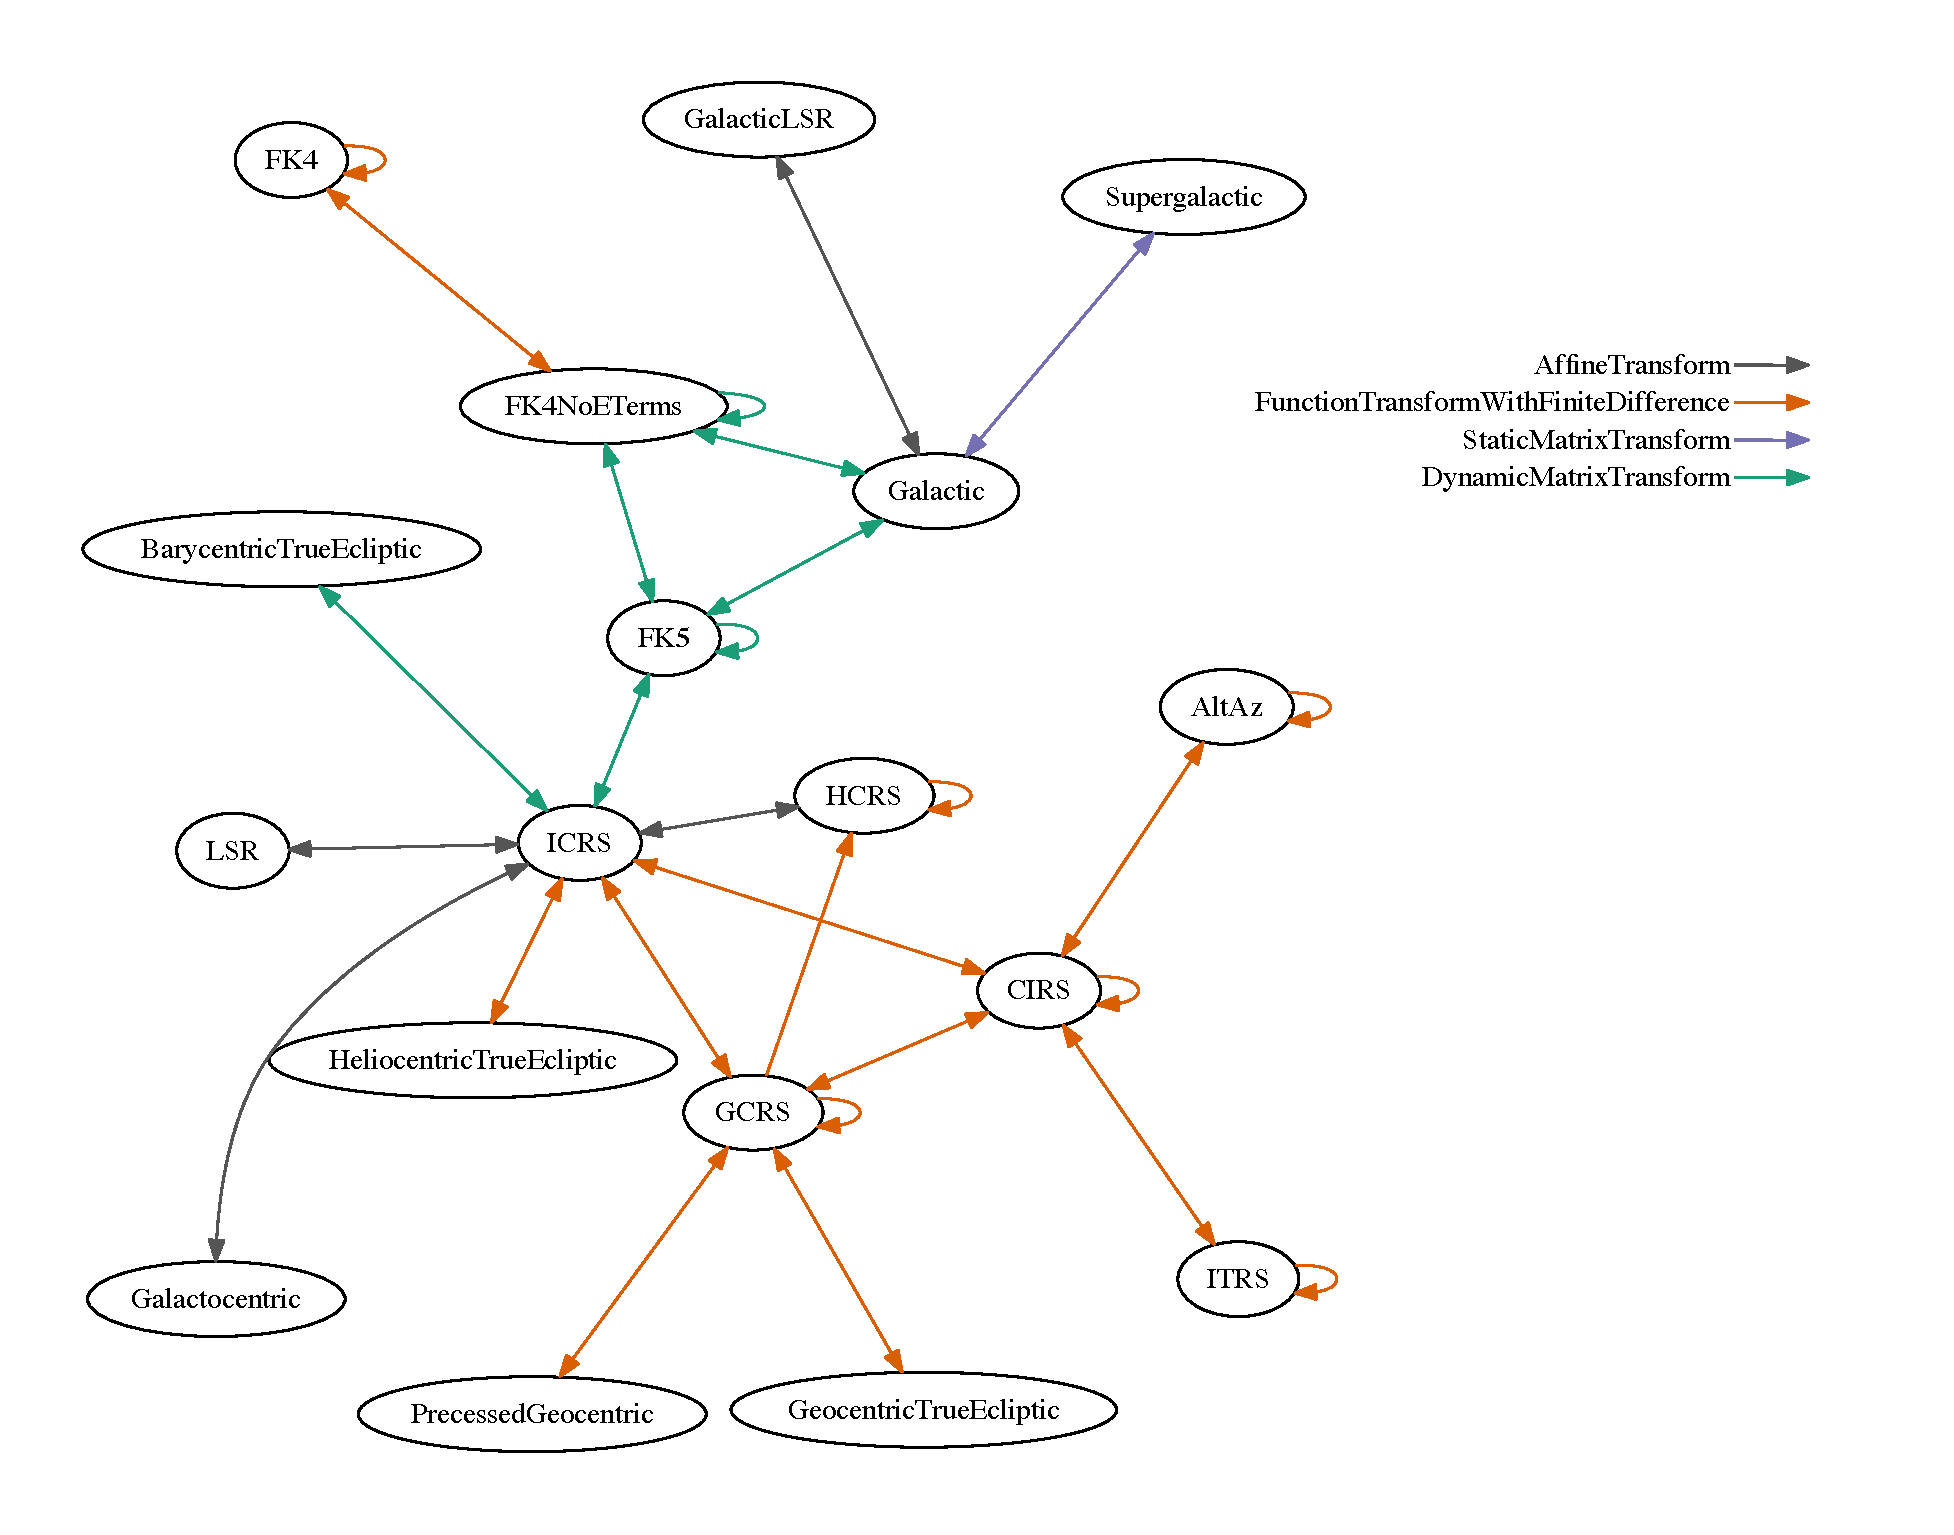
\includegraphics[width=\textwidth]{coordinates_graph.pdf}
\caption{%
    The full graph of possible reference frame transformations implemented in
    \texttt{astropy.coordinates}.
    \label{fig:frame-transform-graph}
}
\end{figure}

The typical user doesn't usually have to interact with the \texttt{Frame} or
\texttt{Representation} classes directly.
Instead, \texttt{astropy.coordinates} provides a high-level interface to
representing astronomical coordinates through the \texttt{SkyCoord} class.
The \texttt{SkyCoord} class was designed to provide a single class that
accepts a wide range of possible inputs.
It supports coordinate data in any coordinate frame in any representation by
internally using the \texttt{Frame} and \texttt{Representation} classes.

In what follows, we briefly highlight key new features in
\texttt{astropy.coordinates}.

\subsubsection{Local Earth coordinate frames}
In addition to representing celestial
    coordinates, \astropypkg now supports specifying positions on the Earth in
    a number of different geocentric systems with the \texttt{EarthLocation}
    class.
    With this, \astropypkg now supports Earth-location-specific coordinate
    systems such as the altitude-azimuth (\texttt{AltAz}) or horizontal system.
    Transformations between \texttt{AltAz} and any Barycentric coordinate frame
    also requires specifying a time using the \texttt{Time} class from
    \texttt{astropy.time}.
    With this new functionality, many of the common tasks associated with
    observation planning can now be completed with \astropypkg or the
    \astropy-affiliated package \package{astroplan}\citep{astroplan_AAS}.

\subsubsection{Proper motion and velocity transformations}
    In addition to positional coordinate data, the \texttt{Frame} classes now
    also support velocity data.
    As the default representation for most frames is spherical, most of the
    \texttt{Frame} classes expect proper motion and radial velocity components
    to specify the velocity information.
    The names of the proper motion components all start with \texttt{pm} and
    adopt the same longitude and latitude names as the positional components.
    Transforming coordinates with velocity data is also supported, but in some
    cases the transformed velocity components have limited accuracy because the
    transformations are done numerically.
    The visualization of the coordinate frame transform graph highlights which
    velocity transformations can be done exactly and which transformations are
    done using a finite-difference scheme.
    The low-level interface for specifying and transforming velocity data (see
    the next point) is currently experimental.
    As such, in v2.0, only the \texttt{Frame} classes (and not the
    \texttt{SkyCoord} class) support handling velocities.

%\subsubsection{Derivatives of coordinate representations}

%\inlinecomment{Tom R}{does this really warrant a separate section or is it just a byproduct of the velocity stuff that can be mentioned in 3.3.2?}

    %As mentioned above, the \texttt{Representation} classes act like
    %three-dimensional vectors.
    %\texttt{astropy.coordinates} now also supports handling first derivatives of
    %vectors / representations through the new \texttt{Differential} classes.
    %The \texttt{Differential} classes are currently used internally within the
    %\texttt{Frame} classes to store the velocity data.

\subsubsection{Solar System Ephemerides}
    Also new is support for computing ephemerides of major solar system bodies
    and outputting the resulting positions as coordinate objects.
    These ephemerides can be computed either using analytic approximations from
    ERFA, or from downloaded JPL ephemerides (the latter requires the
    \package{jplephem}\footnote{\url{https://github.com/brandon-rhodes/python-jplephem}}
    optional dependency and an internet connection).
    % hamogu: I think the specific names of functions can be in the docs
    % and don't need to be repeated here.
    %The \texttt{get\_body} and \texttt{get\_body\_barycentric} functions provide
    %the gateway to this functionality, yielding \texttt{SkyCoord} objects given
    %a specific body and choice of ephemeris source.


\subsubsection{Accuracy of coordinate transformations}

In order to check the accuracy of the coordinate transformations in \package{astropy.coordinates}, we have created a set of benchmarks that we use to compare transformations between a set of coordinate frames for a number of packages\footnote{\url{http://www.astropy.org/coordinates-benchmark/summary.html}}. Since
no package can be guaranteed to implement all transformations to arbitrary precision, and since some transformations are sometimes subject to interpretation of standards (in particular in the case of Galactic coordinates), we do not designate any of the existing packages as the `ground truth' but instead compare each tool to all other tools. The benchmarks are thus useful beyond the \astropy project since they allow all of the tools to be compared to all other tools. The tools included in the benchmark at the moment include the \astropypkg core package, Kapteyn \citep{kapteyn}, NOVAS \citep{novas}, PALpy \citep{pal}, PyAST \citep[a wrapper for AST, described in][]{ast}, PyTPM\footnote{\url{https://github.com/phn/pytpm}}, PyEphem \citep{pyephem}, and pySLALIB \citep[a Python wrapper for SLALIB, described in][]{slalib}.

The benchmarks are meant to evolve over time and include an increasing variety of cases. At the moment, the benchmarks are set up as follows - we have generated a standard set of 1000 pairs of random longitudes/latitudes that we use in all benchmarks. Each benchmark is then defined using an input and output coordinate frame, using all combinations of FK4, FK5, Galactic, ICRS and Ecliptic frames. For now we set the epoch of observation to J2000, and the frame to J2000 in the case of the FK5 and ecliptic frames and B1950 for the FK4 frame, but in future we plan to include a larger variety of epochs and equinoxes, as well as tests of conversion to/from Altitude/Azimuth. For each benchmark, we convert the 1000 longitudes/latitudes from the input/output frame with all tools and quantify the comparison by looking at the median, mean, maximum, and standard deviation of the absolute separation of the output coordinates from each pair of tools. \tablename~\ref{tab:coordinate_benchmarks} gives an example of the relative accuracy of the conversion from FK4 to Galactic coordinates for all pairs of tools. This shows for example that \astropy, Kapteyn and PyTPM agree perfectly (to the precision shown), while PALpy, pySLALIB, and PyAST also agree perfectly amongst themselves, but show an offset of around 0.2\arcsec with the former three packages. Finally, PyEphem disagrees with other packages by 0.4--0.8\arcsec. These values are only meant to be illustrative and will change over time as the benchmarks are refined and packages are updated.
%\inlinecomment{Perry G}{Wouldn't the table be better represented as a matrices? Or perhaps as a matrix as a crude image with colors or intensities representing the size of the quantity. Is the difference between median and mean significant enough to warrant showing both? A link to the actual numbers may satisfy readers that want the exact values, but I suspect the majority don't need to see that precision.}
\begin{table}
\begin{center}
\begin{tabular}{llcccc}
\hline
\hline
Package 1 & Package 2 & Median & Mean & Maximum & Std. Dev. \\
          &           & arcsec & arcsec & arcsec & arcsec \\
\hline
astropy  &  kapteyn  & 0.000  & 0.000 & 0.000 & 0.000 \\
\nodata  &  palpy    & 0.218  & 0.196 & 0.249 & 0.056 \\
\nodata  &  pyast    & 0.218  & 0.196 & 0.249 & 0.056 \\
\nodata  &  pyephem  & 0.459  & 0.458 & 0.860 & 0.231 \\
\nodata  &  pyslalib & 0.218  & 0.196 & 0.249 & 0.056 \\
\nodata  &  pytpm    & 0.000  & 0.000 & 0.000 & 0.000 \\
kapteyn  &  palpy    & 0.218  & 0.196 & 0.249 & 0.056 \\
\nodata  &  pyast    & 0.218  & 0.196 & 0.249 & 0.056 \\
\nodata  &  pyephem  & 0.459  & 0.458 & 0.860 & 0.231 \\
\nodata  &  pyslalib & 0.218  & 0.196 & 0.249 & 0.056 \\
\nodata  &  pytpm    & 0.000  & 0.000 & 0.000 & 0.000 \\
palpy    &  pyast    & 0.000  & 0.000 & 0.000 & 0.000 \\
\nodata    &  pyephem  & 0.563  & 0.570 & 1.012 & 0.253 \\
\nodata    &  pyslalib & 0.000  & 0.000 & 0.000 & 0.000 \\
\nodata    &  pytpm    & 0.218  & 0.196 & 0.249 & 0.056 \\
pyast    &  pyephem  & 0.563  & 0.570 & 1.012 & 0.253 \\
\nodata    &  pyslalib & 0.000  & 0.000 & 0.000 & 0.000 \\
\nodata    &  pytpm    & 0.218  & 0.196 & 0.249 & 0.056 \\
pyephem  &  pyslalib & 0.563  & 0.570 & 1.012 & 0.253 \\
\nodata  &  pytpm    & 0.459  & 0.458 & 0.860 & 0.231 \\
pyslalib &  pytpm    & 0.218  & 0.196 & 0.249 & 0.056 \\
\hline
\end{tabular}
\end{center}
\caption{Comparison of the accuracy of the FK4 to Galactic transformation between different packages.\label{tab:coordinate_benchmarks}}
\end{table}

\subsection{Time}
\label{sec:time}
% Adrian PW

The \package{astropy.time} subpackage focuses on supporting time scales (e.g.,
UTC, TAI, UT1) and time formats (e.g., Julian date, modified Julian date) that
are commonly used in astronomy.
This functionality is needed, for example, to calculate barycentric corrections
or sidereal times.
\package{astropy.time} is currently built on the ERFA (\citealt{erfa}) C
library, which replicates the Standards of Fundamental Astronomy (SOFA;
\citealt{sofa}) but is licensed under a three-clause BSD license.
The package was described in detail in  \citet{astropy} and has
stayed stable for the last several versions of \astropypkg.
Thus, in what follows, we only highlight significant changes or new features
since the previous \astropy paper.


\subsubsection{Barycentric and Heliocentric corrections}
Detailed eclipse or transit
        timing requires accounting for light travel time differences from the
        source to the observatory because of the Earth's motion.
        It is therefore common to instead convert times to the Solar System
        barycenter or heliocenter where the relative timing of photons is
        standardized.
        With the location of a source on the sky (i.e. a \texttt{SkyCoord}
        object), the location of an observatory on Earth (i.e. an
        \texttt{EarthLocation} object), and time values as \texttt{Time}
        objects, the time corrections to shift to the solar system barycenter or
        heliocenter can now be computed with \package{astropy.time} using the
        \texttt{light\_travel\_time} method of a \texttt{Time} object.

\subsection{Data containers}

\subsubsection{\package{nddata}}

The \package{astropy.nddata} subpackage provides three types of functionality: an
abstract interface for representing generic arbitrary-dimensional datasets
intended primarily for subclassing by developers of other packages, concrete
classes building on this interface, and utilities for manipulating these kind of
datasets.

The \texttt{NDDataBase} class provides the abstract interface for gridded data
with attributes for accessing metadata, the world-coordinate system (WCS),
uncertainty arrays matched to the data shape, and other traits.
Building on this interface, the \texttt{NDData} class provides a minimal working implementation for storing \package{numpy} arrays. These classes serve as useful base classes for package authors wishing to develop their own classes for specific use cases and as containers for exchanging gridded data.

The classes \texttt{NDDataRef}, \texttt{NDDataArray}, and \texttt{CCDData} extend the base storing functionality with options to do basic arithmetic (addition, subtraction, multiplication, and division) including error propagation in limited cases and slicing of the dataset based on grid coordinates that appropriately handles masking, errors, and units (if present). Additionally, the \texttt{CCDData} class also provides reading and writing from and to FITS files and uses data structures from \astropypkg, like \texttt{WCS}, to represent the contents of a file abstractly.

The \package{astropy.nddata.utils} module provides utilities that can operate on either plain \package{numpy} arrays or any of the classes in the \package{astropy.nddata} subpackage. It features a class for representing two-dimensional image cutouts, allowing one to easily link pixels in the cutout to pixels in the original image or from the image to the cutout, to convert between world and pixel coordinates in the cutout, and to overlay the cutout on images. Functions to enlarge or reduce an image by doing block replication or reduction are also provided.

\subsubsection{Tables}
\label{sec:table}
% fleshed out / edited by Adrian PW

The \package{astropy.table} subpackage provides functionality for representing
and manipulating heterogeneous data.
%\inlinecomment{APW:}{Need more introduction to the table subpackage!}
The package was described in detail in \cite{astropy}.

Next, we summarize key new features or updates to \package{astropy.table}.

%\inlinecomment{Perry G}{Some mention that some of these are inspired by Pandas?}

\subsubsection{Support for grouped table operations}

A table can contain data that naturally forms groups -- for example it may
contain multiple observations of a few sources at different points in time
and in different bands. We may then want to split the table into groups based
on the combination of source observed and the band, and then combine the
results for each combination of source and band in some way (for example finding
the mean or standard deviation of the fluxes or magnitudes over time) or filter
the groups based on user-defined criteria. These kinds of grouping and
aggregation operations are now fully supported by \texttt{Table} objects.

\subsubsection{Support for table concatenation}

\texttt{Table} objects can now be combined in several different ways. If two
tables have the same columns, we may want to stack them ``vertically'' to create a
new table with the same columns but all rows. If two tables are row-matched but
have distinct columns, we may want to stack them ``horizontally'' to create a
new table with the same rows but all columns. For other situations, more general
table concatenations or joins are also possible when two tables share some
common columns.

\subsubsection{Using astropy objects in tables}

The \texttt{Table} object now allows \texttt{Quantity} objects, celestial
coordinate objects (\texttt{SkyCoord}), and date/time objects (\texttt{Time}) to
be used as columns, and also provides a general way for other user-defined
objects to be used as columns. This makes it possible for example to easily
represent catalogs of sources or time series as in Astropy, and having both the
benefits of the \texttt{Table} object (such as accessing specific rows/columns
or groups of rows/columns, combining tables, and so on) and the benefits of e.g.
the \texttt{SkyCoord} or \texttt{Time} classes (such as converting the
coordinates to a different frame, or accessing the date/time as a modified
Julian date or in another time scale).

\subsection{\package{io}}
% Simon

The \package{astropy.io} subpackage provides support for reading and writing
data to a variety of ASCII and binary file formats, such as a wide range of
ASCII data table formats, FITS, and VOTable.
It also provides a unified interface for reading and writing data with these
different formats using the \package{astropy.table} subpackage.
For many common cases this simplifies the process of file input and output and
reduces the need to master the separate details of all the I/O packages within
\astropypkg.

%\inlinecomment{SCO}{Table and FITS tables}

%\subsubsection{Unified file read/write interface}

%\inlinecomment{Check when it was added (0.3?). Overview of the supported formats (ASCII,FITS, votable, HTML, JSViewer/Datatables).}

% We summarize key new features or updates to \package{astropy.io} below,
% organized by sub-subpackage.

% \inlinecomment{Tom R}{is a sub-subpackage a thing, or is it just 'subpackage' all the way down?}

\subsubsection{ASCII}
% \subsubsection{Enhanced CSV format}

One of the problems when storing a table in an ASCII format is
preserving table meta-data such as comments, keywords and column data
types, units, and descriptions. The newly defined \emph{Enhanced
Character Separated Values} (ECSV,  \citealt{ape6}) format makes it
possible to write a table to an ASCII-format file and read it back
with no loss of information. The ECSV format has been designed to be
both human-readable and compatible with most simple CSV readers.

% \subsubsection{\texttt{.ascii}: fast readers and writers}

The \package{astropy.io.ascii} subpackage now includes a significantly faster
Cython/C engine for reading and writing ASCII files. This is available for the
most common formats.  On average the new engine is about 4 to 5 times faster
than the corresponding pure-\python implementation, and is often comparable to
the speed of the \package{Pandas} \citep{pandas} ASCII file interface.  The
fast reader has parallel processing option that allows harnessing multiple
cores for input parsing to achieve even greater speed gains.  By default,
\texttt{read()} and \texttt{write()} will attempt to use the fast C engine
when dealing with compatible formats. Certain features of the full read
/ write interface are not available in the fast version, in which case the
pure-\python version will automatically be used.

% \subsubsection{\texttt{.ascii}: HTML tables}

The \package{astropy.io.ascii} subpackage now provides the capability
to read a table within an HTML file or web URL into an astropy
\texttt{Table} object. Conversely a \texttt{Table} object can now
be written out as an HTML table.

\subsubsection{FITS}

The \package{astropy.io.fits} subpackage started as a direct port of the
PyFITS project \citep{PyFITS}. Therefore it is pretty stable, with mostly bug
fixes but also a few new features and performance improvements.  The API
remains compatible with PyFITS, which is now deprecated in favor of
\astropypkg.

Command-line scripts are now available for printing a summary of the HDUs in
a FITS file(s) (\texttt{fitsinfo}) and for printing the header information to
the screen in a human-readable format (\texttt{fitsheader}).

FITS files are now loaded \emph{lazily} (the default behavior, which can be
deactivated if needed), where all HDUs are not loaded until they are
requested. This should provide substantial speedups for situations using the
convenience functions (e.g., \texttt{getheader()} or \texttt{getdata()}) to
get HDU’s that are near the front of a file with many HDUs.

% \inlinecomment{Tom R}{too detailed? I don't think we need to mention every single performance enhancement, right?}

% \subsubsection{\texttt{.misc}: YAML serialization}

% The new \package{astropy.io.misc.yaml} module allows converting astropy
% objects into a standard YAML format.  This can be used beyond
% \texttt{astropy.io.misc.yaml}: for example, to serialize the metadata of
% tables before saving to other formats like HDF5.


%\inlinecomment{BMS}{Maybe move the command line tools into a separate subsection to highlight them (even though we mostly only have fits related scripts)? They are supposed to be used more frequently by individual users.}
%\inlinecomment{hamogu}{MY feeling is that this section is too detailed already. If I had written it, I would not have mentioned the scripts at all.}

\subsection{Modeling}
\label{sec:modeling}
% The whole modeling submodule was missing from the previous paper, so everything really, including compound models, unit support etc.
% Nadia, Lim
% Tom R. -- unit support
\subsubsection{Overview}
The \package{astropy.modeling} subpackage provides a framework for representing
analytical models and performing model evaluation and parameter fitting. Models and
fitters are independent of each other: a model can be fit with different
fitters and new fitters can be added without changing existing models. The
framework is designed to be flexible and easily extensible. The goal is to have
a rich set of models but also make it easy to create new ones if necessary. The
modeling framework is used in a variety of data analysis tools and is the basis
for the Generalized World Coordinate System (GWCS)
package.\footnote{\url{https://github.com/spacetelescope/gwcs}}

% hamogu: I comented this out because we don't have prrof that it's
% ``uniquly'' useful. THe developers of e.g. ISIS, Sherpa, for even IRAF
% will probably disagree.
%The recently-added support for \package{astropy.units} in models and fitters
%make it a uniquely powerful package for working with astrophysical models.

\subsubsection{Single Model Definition and Evaluation}

%\inlinecomment{hamogu: I tihnk this is too techical. I know it's a complex subpackage but I had trouble understanding this section even as a regular user.}

Most models are defined by parameters and maintain an ordered list of parameter names, \texttt{Model.param\_names}. A model is instantiated by passing in values (scalars or arrays) for its parameters. A parameter is a descriptor that provides a proxy for the value and stores additional information -- default value, default unit, and parameter constraints. The value and constraints can be updated by assignment. Supported parameter constraints include \texttt{fixed}, and \texttt{tied} parameters, and \texttt{bounds} on parameter values. Most models have a fixed parameter set but for some (e.g., polynomials), the number of parameters is defined by another argument (e.g., degree-of-freedom in the case of polynomials). Parameters support arithmetic operations and are combined with the inputs during evaluation using the \package{numpy} broadcasting rules. A model is evaluated by calling it as a function.

Models have a \texttt{Model.inverse} property, which returns the analytical inverse, if available, or raises an exception otherwise. This is a settable property; i.e. a model instance can be assigned as inverse to another model. For example, a polynomial model can be assigned as an inverse to another polynomial model.

Another useful settable property of models is \texttt{Model.bounding\_box}. This attribute sets the domain over which the model is defined. This greatly improves the efficiency of evaluation when the input range is much larger than the characteristic width of the model itself.

\subsubsection{Model Sets}

\package{astropy.modeling} provides an efficient way to instantiate the same type of model with many different sets of parameter values by passing the \texttt{n\_models} argument on instantiation, which sets the number of models to instantiate. This creates a model set that can be efficiently evaluated for example, in PSF (point spread function) photometry, all objects in an image will have a PSF of the same functional form, but with different positions and amplitudes.

\subsubsection{Compound Models}
Models can be combined using arithmetic expressions. The result is also a model, which can further be combined with other models. Modeling supports arithmetic (+, -, *, /, and **), join ($\&$), and composition ($|$) operators. The rules for combining models involve matching their inputs and outputs. For example, the composition operator, $|$, requires the number of outputs of the left model to be equal to the number of inputs of the right one. For the join operator, the total number of inputs must equal the sum of number of inputs of both the left and the right models. For all arithmetic operators, the left and the right models must have the same number of inputs and outputs. An example of a compound model could be a spectrum with interstellar absorption. The stellar spectrum and the interstellar extinction are represented by separate models, but the observed spectrum is fitted with a compound model that combines both.

\subsubsection{Fitting Models to Data}

\package{astropy.modeling} provides several fitters which are wrappers around some of the \texttt{numpy} and \texttt{scipy.optimize} functions and provide support for specifying parameter constraints. The fitters take a model and data as input and return a copy of the model with the optimized parameter values set. The goal is to make it easy to extend the fitting framework to create new fitters. The optimizers available in \astropypkg version 2.0 are Levenberg--Marquardt, Simplex, SLSQP, and LinearLSQFitter (which is based on \texttt{numpy.linalg} that provides exact solution for linear models).

%\inlinecomment{APW}{Add citations for the different optimizaton algorithms in paragraph above?}

Modeling also supports a plugin system for fitters, which allows using the
\astropypkg models with external fitters. An example of this is
\package{SABA}\footnote{\url{https://github.com/astropy/saba}}, which is a bridge between
Sherpa\footnote{\url{http://cxc.cfa.harvard.edu/contrib/sherpa/}}
and \package{astropy.modeling}, to bring the Sherpa fitters into \astropypkg.

\subsubsection{Creating New Models}

New model classes can be created in two ways:
\begin{enumerate}
   \item The simplest way is to use the \texttt{custom\_model} decorator in modeling with a user-defined function that takes the inputs and model parameters as arguments.
   \item It is also possible to create an arbitrarily complex custom model based on the \texttt{Model} class.
\end{enumerate}

\subsubsection{Unit Support}

The \package{astropy.modeling} subpackage now supports the representation, evaluation, and fitting of models using \texttt{Quantity} objects, which attach units to scalar values or arrays of values. In practice, this means that one can, for example, fit a model to data with units and get parameters that also have units out, or initialize a model with parameters with units and evaluate it using input values with different but equivalent units. Using this, we have implemented a blackbody model (\texttt{BlackBody1D}) that can be used to fit observed fluxes in a variety of units and as a function of different units of spectral coordinates (e.g., wavelength or frequency).

\subsection{Convolution}
% Adam G.

The \package{astropy.convolution} subpackage implements `normalized convolution' \citep[e.g.,][]{Knutsson1993}, which is an image reconstruction technique in which missing data are ignored during the convolution and replaced with values interpolated using the kernel.   An example of this is given in \figurename~\ref{fig:convolution-example}.  In versions $\leq 1.3$, the direct convolution and Fast Fourier Transform (FFT) convolution approaches were not consistent, with FFT convolution implementing normalized convolution and direct convolution implementing a different approach.  As of version 2.0, the two methods are consistent and include a suite of consistency checks.

\begin{figure}
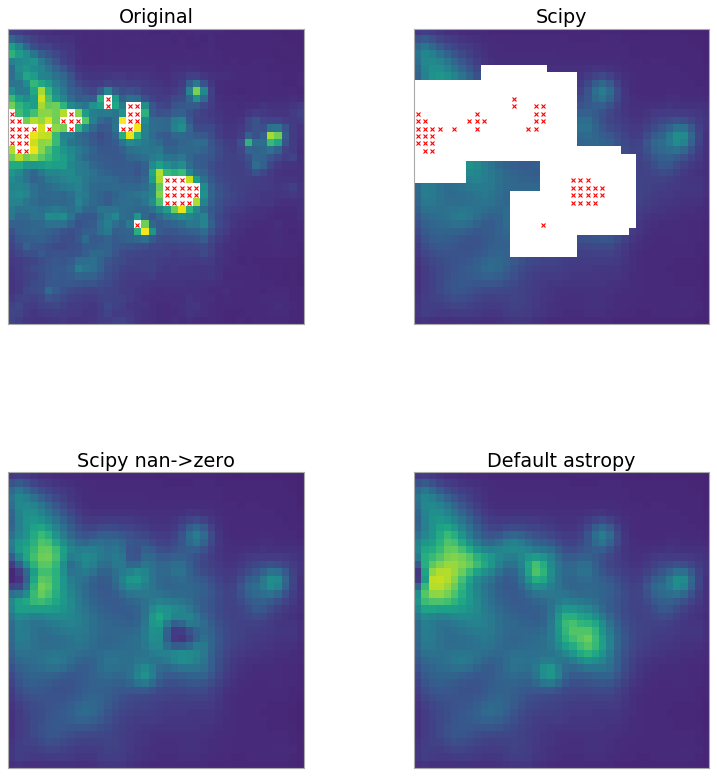
\includegraphics[width=\textwidth]{convolution_example.png}
\caption{%
    An example showing different modes of convolution available in the \python
    ecosystem.  The red x's mark pixels that are set to NaN in the original data
    (a).  If the data are convolved with a Gaussian kernel on a $9\times 9$ grid using
    scipy's direct convolution (b), any pixel within range of the original NaN
    pixels is also set to NaN.  Panel (c) shows what happens if the NaNs are set
    to zero first: the originally NaN regions are depressed relative to their
    surroundings.  Finally, panel (d) shows \astropypkg's convolution behavior,
    where the missing pixels are replaced with values interpolated from their
    surroundings using the convolution kernel.
    \label{fig:convolution-example}
}
\end{figure}


\subsection{Visualization}
% Larry:  Image visualization (stretching, scaling), RGB

The \package{astropy.visualization} subpackage provides functionality that can be helpful when visualizing data. This includes a framework for plotting astronomical images with coordinates with \package{matplotlib} (previously the standalone \package{wcsaxes} package), functionality related to image normalization (including both scaling and stretching), smart histogram plotting, RGB color image creation from separate images, and custom plotting styles for \package{matplotlib}.

\subsubsection{Image Stretching and Normalization}

\label{sec:stretch}

\package{astropy.visualization} provides a framework for transforming values in images (and more generally any arrays), typically for the purpose of visualization. Two main types of transformations are normalization and stretching of image values.

Normalization transforms the images values to the range $[0,1]$ using lower and upper limits $(v_{\rm min}, v_{\rm max})$
\begin{equation}
y = \frac{x - v_{\rm min}}{v_{\rm max} - v_{\rm min}}
\end{equation}
where $x$ represents the values in the original image.

Stretching transforms the image values in the range $[0,1]$ again to the range $[0,1]$ using a linear or non-linear function
\begin{equation}
z = f(y) \quad .
\end{equation}

Several classes are provided for automatically determining intervals (e.g., using image percentiles) and for normalizing values in this interval to the $[0,1]$ range.

\package{matplotlib} allows a custom normalization and stretch to be used when displaying data by passing a normalization object. The \package{astropy.visualization} package also provides a normalization class that wraps the interval and stretching objects into a normalization object that \package{matplotlib} understands.

\subsubsection{Plotting image data with world coordinates}

Astronomers dealing with observational imaging commonly need to make figures with images that include the correct coordinates and optionally display a coordinate grid. The challenge, however, is that the conceptual coordinate axes (such as longitude/latitude) need not be lined up with the pixel axes of the image. The \package{astropy.visualization.wcsaxes} subpackage implements a generalized way of making figures from an image array and a world coordinate system (WCS) object that provides the transformation between pixel and `world' coordinates.

World coordinates can be, for example, right ascension and declination, but can also include, for example, velocity, wavelength, frequency, or time. The main features from this subpackage include the ability to control which axes to show which coordinate on (for example showing longitude ticks on the top and bottom axes and latitude on the left and right axes), controlling the spacing of the ticks either by specifying the positions to use or providing a tick spacing or an average number of ticks that should be present on each axis, setting the format for the tick labels to ones commonly used by astronomers, controlling the visibility of the grid/graticule, and overlaying ticks, labels, and/or grid lines from different coordinate systems. In addition, it is possible to pass data with more than two dimensions and slice on-the-fly. Finally, it is possible to define non-rectangular frames, such as, for example, Aitoff projections.

This subpackage differs from \package{APLpy} \citep{aplpy} in that the latter focuses on providing a very high-level interface to plotting that requires very few lines of code to get a good result, whereas \package{wcsaxes} defines an interface that is much closer to that of \package{matplotlib} \citep{matplotlib}. This enables significantly more advanced visualizations.

An example of a visualization made with \package{wcsaxes} is shown in \figurename~\ref{fig:wcsaxes} -- this example illustrates the ability to overlay multiple coordinate systems and customize which ticks/labels are shown on which axes around the image. This also uses the image stretching functionality from \sectionname~\ref{sec:stretch} to show the image in a square root stretch (automatically updating the tick positions in the colorbar).

\begin{figure}
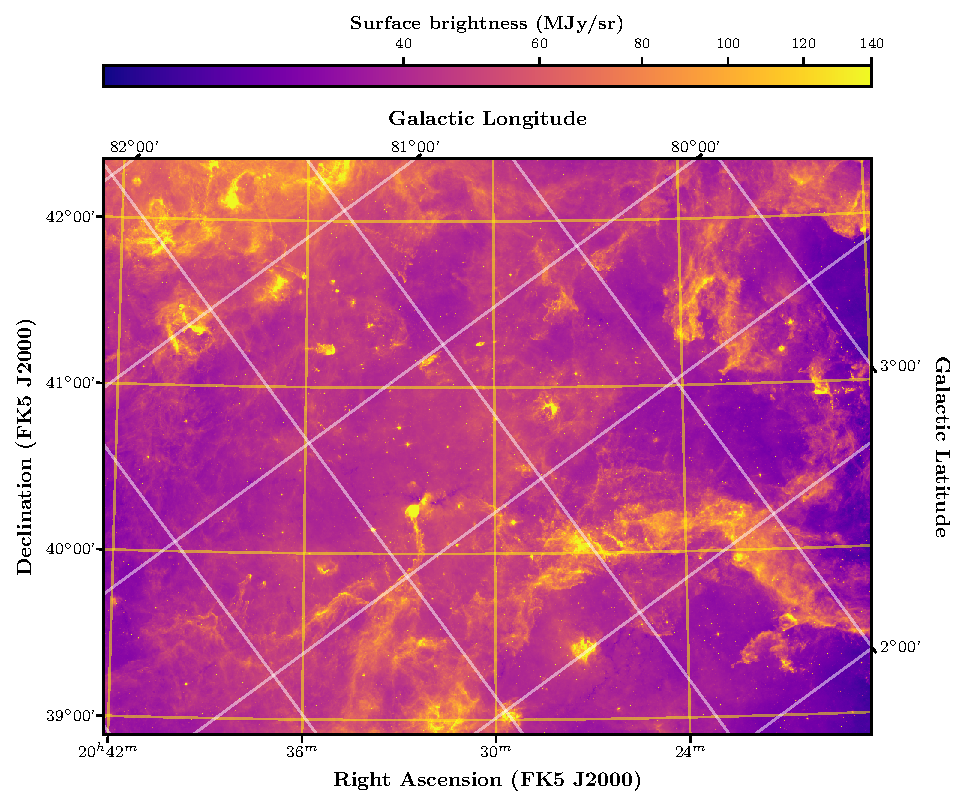
\includegraphics[width=\textwidth]{cygnus_x_spitzer.pdf}
\caption{%
An example of figure made using the \package{astropy.visualization.wcsaxes} subpackage, using \textit{Spitzer}/IRAC 8.0~$\mu$m data from the Cygnus-X \textit{Spitzer} Legacy survey \citep{cygnusx}.
\label{fig:wcsaxes}
}
\end{figure}

\subsubsection{Choosing Histogram Bins}

\package{astropy.visualization} also provides a histogram function, which is a
generalization of \texttt{matplotlib}’s histogram function, to allow for more
flexible specification of histogram bins.  The function provides several methods
of automatically tuning the histogram bin size. It has a syntax identical to
\texttt{matplotlib}’s histogram function, with the exception of the \texttt{bins}
parameter, which allows specification of one of four different methods for
automatic bin selection: `blocks', `knuth', `scott', or `freedman'.

\subsubsection{Creating color RGB images}

\cite{Lupton2004} describe an ``optimal'' algorithm for producing red-green-blue (RGB) composite images from three separate high-dynamic range arrays. The \package{astropy.visualization} subpackage provides a convenience function to create such a color image.  It also includes an associated set of classes to provide alternate scalings.
This functionality was contributed by developers from the Large Synoptic Survey Telescope (LSST) and serves as an example of contribution to \astropy from a more traditional engineering organization \citep{Jennes2016}.

The Sloan Digital Sky Survey (SDSS) SkyServer color images were made using a variation on this technique.  As an example, in \figurename~\ref{fig:ngc6977} we show an RGB color image of the Hickson 88 group, centered near NGC~6977.  This image was generated from SDSS images using the \package{astropy.visualization} tools.

\begin{figure}
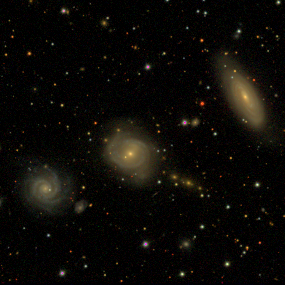
\includegraphics[width=\textwidth]{ngc6977.png}
\caption{An RGB color image of the region near the Hickson 88 group
constructed from SDSS images and the \package{astropy.visualization}
tools.
\label{fig:ngc6977}}
\end{figure}

%\subsection{Utils}
% Lim

\subsection{Cosmology}

The \package{cosmology} package contains classes for representing different cosmologies and functions for calculating commonly used quantities such as look-back time and distance.   The package was described in detail in \cite{astropy}.  The default cosmology in \astropy version 2.0 is given by the values in \cite{2016A&A...594A..13P}.

\subsection{Statistics}
% Edited by Adrian PW

The \package{astropy.stats} package provides statistical tools that
are useful for or specific to astronomy and are not found in or extend
the available functionality of other \python statistics packages such
as \package{scipy} \citep{scipy} or \package{statsmodels}
\citep{seabold2010statsmodels}.  \package{astropy.stats} contains
a range of functionality used by many different disciplines
in astronomy. It is not a complete set of statistic tools, but rather
a still growing collection of useful features.

% The current review process for contributions to the \package{astropy.stats} package includes review of the code, documentation, testing, and scientific merit of the inclusion.  When necessary, scientific reviewers outside of the maintainers will be sought for their input on new pull requests.

In this section, we describe these tools, including robust statistical estimators, circular statistics, periodograms, spatial statistics, and histogram binning.


% Steve C.: overview, circular stats,
% Jake V.:  Lomb-scargle, Bayesian blocks
% Larry:  sigma clipping, biweight stats
% Ze':  Ripley's K (spatial stats)

\subsubsection{Robust Statistical Estimators}

Robust statistics provide reliable estimates of basic statistics for complex distributions that largely mitigate the effects of outliers. \package{astropy.stats} includes several robust statistical functions that are commonly used in astronomy, such as sigma clipping methods for rejecting outliers, median absolute deviation functions, and biweight estimators, which have been used to calculate the velocity dispersion of galaxy clusters \citep{Beers1990}.

\subsubsection{Circular Statistics}

Astronomers often need to compute statistics of quantities evaluated on a circle, such as sky direction or polarization angle.
A set of circular statistical estimators based on \citet{JammalamadakaSengupta}
are implemented in \package{astropy.stats}.  These functions provide
measurements of the circular mean, variance, and moment.   For all of these
functions, they work with both \texttt{numpy.ndarrays} (assumed to be in
radians) and \texttt{Quantity} objects.  In addition, the subpackage includes
tests for Rayleigh Test, vtest, and a function to compute the maximum likelihood
estimator for the parameters of the von Mises distribution.

\subsubsection{Lomb-Scargle Periodograms}

Periodic analysis of unevenly-spaced time series is common across many subfields of astronomy. The \package{astropy.stats} package now includes several efficient implementations of the Lomb-Scargle periodogram \citep{Lomb76, Scargle82} and several generalizations, including floating mean models \citep{Zechmeister09}, truncated Fourier models \citep{Bretthorst2003}, and appropriate handling of heteroscedastic uncertainties. Importantly, the implementations make use of several fast and scalable computational approaches \citep[e.g.,][]{Press89, Palmer09}, and so can be applied to much larger datasets than Lomb-Scargle algorithms available in, e.g., \package{scipy.stats} (\citealt{scipy}). Much of the Lomb-Scargle code in \astropy has been adapted from previously-published open-source code \citep{astroML, VanderPlas2015}.

\subsubsection{Bayesian Blocks and Histogram Binning}
\astropypkg also includes an implementation of {\it Bayesian Blocks} \citep{Scargle2013}, an algorithm for analysis of break-points in non-periodic astronomical time-series. One interesting application of Bayesian Blocks is its use in determining optimal histogram binnings, and in particular binnings with unequal bin sizes. This code was adapted, with several improvements, from the \package{astroML} package \citep{astroML}. An example of a histogram fit using the Bayesian blocks algorithm is shown in the right panel of \figurename~\ref{fig:bayes-blocks-hist}.

\begin{figure}
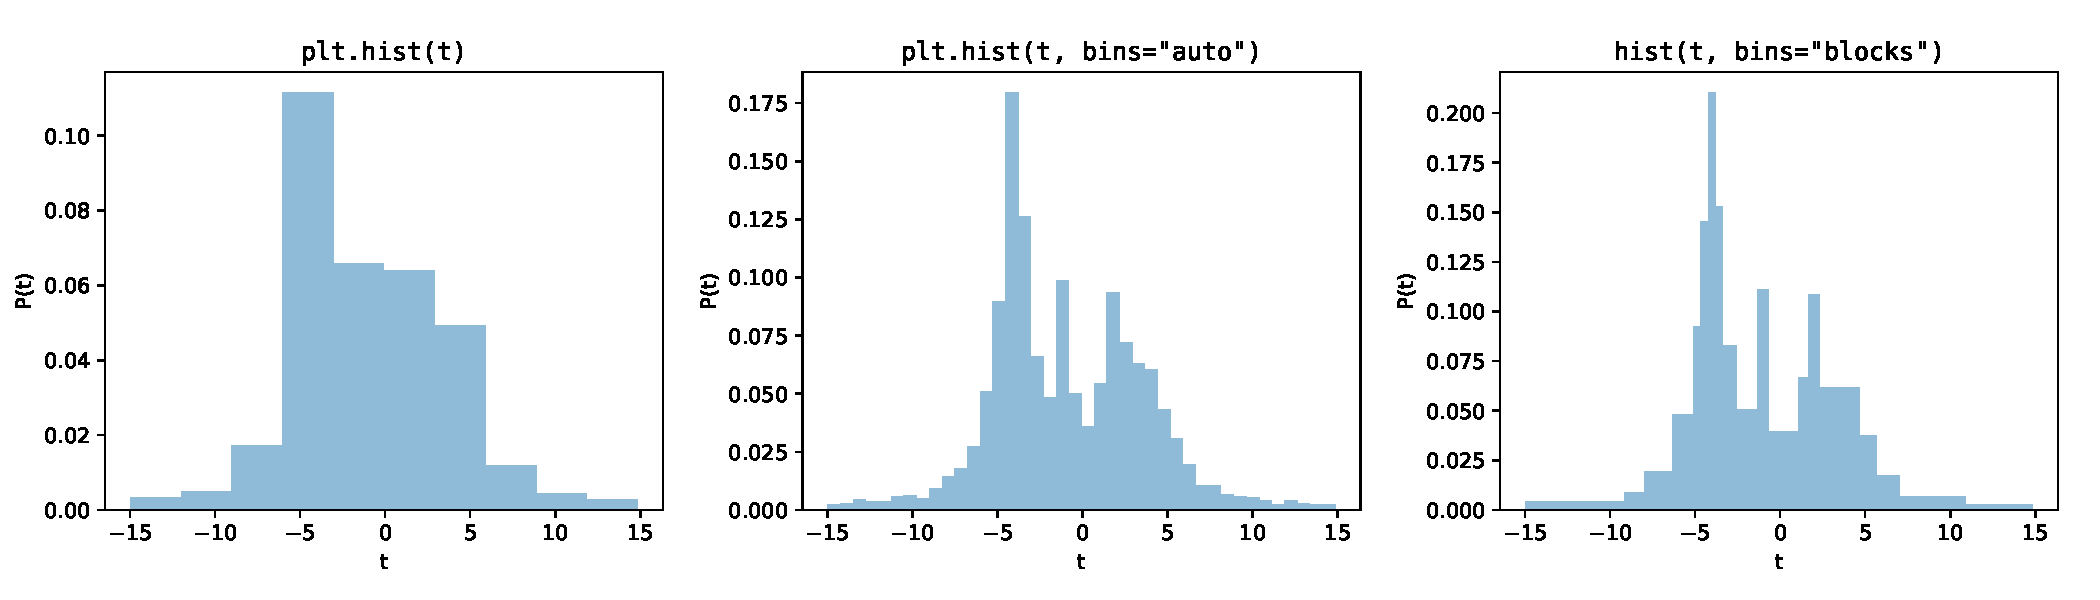
\includegraphics[width=\textwidth]{bayesian_blocks_hist.pdf}
\caption{%
    Three approaches to a 1D histogram:
    {\it left:} a standard histogram using \package{matplotlib}'s default of 10 bins.
    {\it center:} a histogram with the number of equal-width bins determined automatically using \package{numpy}'s {\tt bins='auto'}.
    {\it right:} a histogram created with \package{astropy}, with irregularly-spaced bins computed via the Bayesian Blocks algorithm.
    Compared to regularly-spaced bins, the irregular bin widths give a more accurate visual representation of features in the dataset at various scales.
    \label{fig:bayes-blocks-hist}
}
\end{figure}

\section{Infrastructure for Astropy affiliated packages}

\label{sec:infrastructure}
%\inlinecomment{BMS}{should we describe astropy-helpers even though it's future is unsure?}
% Text also edited by Adrian PW

In addition to astronomy-specific packages and libraries, the \astropy Project
also maintains and distributes several general-purpose infrastructure packages
that help with the maintenance and upkeep of the \astropypkg core package and
other affiliated packages.
The following sections describes the most widely-used infrastructure packages
developed by the \astropy Project.

\subsection{Package template}
% Brigitta may write this up if there is no other takers

\astropy provides a package template --- as a separate \github repository,
\package{astropy/package-template}\footnote{\url{https://github.com/astropy/package-template/}}
--- that aims to simplify setting up packaging, testing, and
documentation builds for developers of affiliated packages or
\astropypkg-dependent packages.
Any \python package can make use of this ready-to-go package layout, setup,
installation, and \package{Sphinx} documentation build infrastructure that was
originally developed for the \astropypkg core package and affiliated packages
maintained by the \astropy project.
The package template also provides a testing framework, template configurations
for continuous integration services, and \package{Cython} build support.

\subsection{Continuous integration helpers}
% Brigitta

\astropy also provides a set of scripts for setting up and configuring
continuous integration (CI) services as a \github repository,
\package{astropy/ci-helpers}.\footnote{\url{https://github.com/astropy/ci-helpers}}
These tools aim to empower package maintainers to control their testing set up
and installation process for various continuous integration services through a
set of environment variables.
While the current development is mostly driven by the needs of the \astropy
ecosystem, the actual usage of this package is extremely widespread. The current
tools support configuration for Travis CI and Appveyor CI.

\subsection{Sphinx extensions}

The documentation for many \python packages, the core \astropypkg package, and
for all packages in the \astropy ecosystem is written using the
\package{Sphinx} documentation build system.
\package{Sphinx} makes it possible to write documentation using plain text files
that follow a markup language called ``reStructuredText,'' which are then
transformed into HTML or \LaTeX{} documentation during the documentation build
process.
For the \astropy project, we have developed a few \package{Sphinx} extensions
that facilitate automatically generating API documentation for large projects,
like the \astropypkg core package.
The main extension we have developed is
\package{sphinx-automodapi}\footnote{\url{http://sphinx-automodapi.readthedocs.io}},
which makes it easy with a single reStructuredText command to generate a set of
documentation pages listing all of the available classes, functions, and
attributes in a given \python module.

%\inlinecomment{TPR}{We should put the releases of sphinx-automodapi on Zenodo and cite this}

% \section{State of the Ecosystem}
% Commenting out unless a clear statement is added

\section{The future of the Astropy project}
\label{sec:future}
% First draft by SMC
% edited by BMS
% edited again by Adrian PW

Following the release of version 2.0, development on the next major version of
the \astropypkg core package (version 3.0) has already begun.
On top of planned changes and additions to the core package, we also plan to
overhaul the \astropy educational and learning materials, and further refactor
and generalize the infrastructure utilities developed for the core package for
the benefit of the community.

%\inlinecomment{BMS}{should we mention the refactored infra here?  e.g. pytest-astropy and sphinx-astropy?}

\subsection{Future versions of the \astropypkg core and affiliated packages}

One of the most significant changes coming in this next major release will be
removing support for \python 2 \citep{ape10}: future versions of \astropypkg
will only support \python 3.5 and higher.
Removing \python 2 support will allow the use of new, \python 3-only features,
will simplify the code base, and reduce the testing overhead for the package.
\astropypkg version 3.0 is currently scheduled for January 2018.

In the next major release after version 3.0, scheduled for the summer of
2018, the focus will be on optimization of the code and improved
documentation.
To prepare for this release, we are preparing software for testing, evaluating,
and monitoring the performance of the code.
Less functionality may be introduced in this release while the focus will be
primarily on improved performance.

Beyond the core code, the \astropy project is also further developing the
\astropy-managed affiliated packages.
While these may not be integrated into the \astropypkg core package, these
projects provide code that is useful to the astronomical community and meet the
testing and documentation standards of \astropy.
Some of these new efforts includes an initiative to develop tools for
spectroscopy \citep[\package{specutils}, \package{specreduc}, \package{specviz}]
{ape13}, integration of LSST software, and packages to support HEALPIX
projection. %\citep{astropy-healpix}
%\inlinecomment{BMS}{TODO: uncomment references of packages once they are available}

\subsection{Learn Astropy}
% Adrian

The \astropypkg core package documentation contains narrative descriptions of
the package functionality along with detailed usage notes for functions,
classes, and modules.
While useful as a reference and for more advanced \python users, it is not the
right entry-point for all users or learning environments.
In the near future, we will launch a new resource for learning to use both the
\astropypkg core package and the many packages in the broader \astropy
ecosystem, under the name `\emph{Learn Astropy}.'

The new \emph{Learn Astropy} site will present several different ways to engage
with the \astropy ecosystem:
\begin{description}
    \item[Documentation] The \astropypkg and affiliated package documentation
        contain the complete description of a package with all requisite
        details, including usage, dependencies, and examples.
        The pages will largely remain as-is, but will be focused towards more
        intermediate users and as a reference resource.
    \item[Examples] These are stand-alone code snippets that live in the
        \astropypkg documentation that demonstrate a specific functionality
        within a subpackage.
        The \astropypkg core package documentation will then gain a new ``index
        of examples'' that links to all of the code or demonstrative examples
        within any documentation page.
    \item[Tutorials] The \astropy tutorials are step-by-step demonstrations of
        common tasks that incorporate several packages or subpackages.
        Tutorials are more extended and comprehensive than examples, may contain
        exercises for the users, and are generally geared towards workshops or
        teaching.
        Several tutorials already
        exist\footnote{\url{http://tutorials.astropy.org/}} and are being
        actively expanded.
    \item[Guides] These are long-form narrative, comprehensive,
        conceptually-focused documents (roughly one book chapter in length)
        providing stand-alone introductions to core packages in addition to the
        underlying astronomical concepts.
        These are less specific and more conceptual than tutorials.
        For example, ``using \astropypkg and \package{ccdproc} to reduce imaging
        data.''
\end{description}
We encourage any users who wish to see specific material to either contribute or
comment on these efforts via the \astropy mailing list or \astropy-tutorials
\github repository.\footnote{\url{https://github.com/astropy/astropy-tutorials}}

\section{Conclusion}
\label{sec:conclusion}
% Renamed and edited by Adrian PW

The development of the \astropypkg package and cultivation of the \astropy
ecosystem is still maintaining significant growth while improving stability,
breadth, and reliability.
As the \astropypkg core package becomes more mature, several subpackages have
reached stability with a rich set of features that help astronomers worldwide to
perform many daily tasks such as planning observations, analyzing data or
simulation results, and writing publications.
The strong emphasis that the \astropy project puts on reliability and code
correctness helps users to trust the calculations performed with \astropypkg and
to publish reproducible results.
At the same time, the \astropy ecosystem and core package are growing: new
functionality is still being contributed, and new affiliated packages are being
developed to support more specialized needs.

The \astropy project is also spreading awareness of best practices in
community-driven software development.
This is important as most practicing astronomers were not explicitly taught
computer science and software development, despite the fact that a major
fraction of nearly every astronomer's workload today is related to software use
and development.
The \astropypkg package leads by example, showing all interested astronomers how
modern tools like \texttt{git} version control or continuous integration can
increase the quality, accessibility, and discoverability of astronomical
software without overly complicating the development cycle.
Within \astropy, all submitted code is reviewed by at least one, but typically
more, members of the \astropy community, who provide feedback to contributors
to help improve their skills.
As a community, we follow an explicit code of conduct \citep{ape8} and treat all
contributors and users with respect, provide a harassment-free environment, and
encourage and welcome new contributions from all.
Thus, while the \astropy project provides and develops software and tools
essential to modern astronomical research, it also helps to prepare the current
and next generation of researchers with the knowledge to adequately use,
develop, and contribute to those tools within a conscientious and welcoming
community.

\acknowledgments The \astropy community is supported by and makes use
of a number of organizations and services outside the traditional
academic community. We thank Google for financing and organizing the
Google Summer of Code (GSoC) program, that has funded severals
students per year to work on \astropy related projects over the
summer. These students often turn into long-term contributors. We also
thank NumFOCOS and the Python Software Foundation for financial
support. Within the academic community, we thank
institutions that make it possible that developers on
their staff can contribute their time to the development of
\astropy projects.

Furthermore, the \astropy packages would not exist
in their current form without a number of web services for code
hosting, continuous integration, and documentation; in particular,
\astropy heavily relies on GitHub, Travis CI, Appveyor, CircleCI, and
Read the Docs.

\astropypkg interfaces with the SIMBAD database,
operated at CDS, Strasbourg, France. It also makes use of the ERFA library \citep{erfa}, 
which in turn derives from the IAU SOFA Collection\footnote{http://www.iausofa.org} developed by the International Astronomical Union Standards of Fundamental Astronomy \citep{sofa}.

\software{\package{astropy} (\citealt{astropy}),
          \package{numpy} (\citealt{numpy}),
          \package{scipy} (\citealt{scipy}),
          \package{matplotlib} (\citealt{matplotlib}),
          \package{Cython} (\citealt{cython}),
          \package{SOFA} (\citealt{sofa}),
          \package{ERFA} (\citealt{erfa})
          }

\bibliographystyle{aasjournal}
\bibliography{bibliography}


\appendix
\section{List of Affiliated Packages}

%\inlinecomment{SMC}{Can a brief description of each code be added?}

\begin{longrotatetable}
  \begin{deluxetable*}{ccccc}
    \tablecaption{Registry of affiliated packages.}
    \label{tab:registry}
    \tablehead{
        \colhead{Package Name} &
        \colhead{Stable} &
        \colhead{PyPI Name} &
        \colhead{Maintainer} &
        \colhead{Citation}
      }
      \startdata
        \href{https://github.com/astropy/astroscrappy}{Astro-SCRAPPY} & Yes & \href{https://pypi.python.org/pypi/astroscrappy}{astroscrappy} & Curtis McCully & \citealt{astroscrappy} \\
\href{https://github.com/astropy/astroplan}{astroplan} & No & \href{https://pypi.python.org/pypi/astroplan}{astroplan} & Brett Morris & \citealt{astroplan_AAS}\\
\href{http://github.com/astropy/astroquery}{astroquery} & Yes & \href{https://pypi.python.org/pypi/astroquery}{astroquery} & Adam Ginsburg and Brigitta Sipocz & \citealt{astroquery}\\
\href{http://github.com/astropy/ccdproc}{ccdproc} & Yes & \href{https://pypi.python.org/pypi/ccdproc}{ccdproc} & Steven Crawford, Matt Craig, and Michael Seifert & \citealt{ccdproc}\\
\href{https://github.com/jesford/cluster-lensing}{cluster-lensing} & No & \href{https://pypi.python.org/pypi/cluster-lensing}{cluster-lensing} & Jes Ford & \citealt{clusterlensing} \\
\href{https://github.com/adrn/gala}{gala} & Yes & \href{https://pypi.python.org/pypi/astro-gala}{astro-gala} & Adrian Price-Whelan & \citealt{gala}\\
\href{https://github.com/jobovy/galpy}{galpy} & Yes & \href{https://pypi.python.org/pypi/galpy}{galpy} & Jo Bovy & \citealt{galpy}\\
\href{http://github.com/gammapy/gammapy}{gammapy} & No & \href{https://pypi.python.org/pypi/gammapy}{gammapy} & Christoph Deil & \citealt{gammapy}\\
\href{http://github.com/ejeschke/ginga}{ginga} & Yes & \href{https://pypi.python.org/pypi/ginga}{ginga} & Eric Jeschke and Pey-Lian Lim & \citealt{ginga}\\
\href{https://github.com/glue-viz/glue}{Glue} & Yes & \href{https://pypi.python.org/pypi/glueviz}{glueviz} & Chris Beaumont and Thomas Robitaille & \citealt{glue}\\
\href{https://github.com/spacetelescope/gwcs}{gwcs} & No & \href{https://pypi.python.org/pypi/gwcs}{gwcs} & Nadia Dencheva & \citealt{gwcs}\\
\href{https://github.com/astropy/halotools}{Halotools} & Yes & \href{https://pypi.python.org/pypi/halotools}{halotools} & Andrew Hearin & \citealt{halotools}\\
\href{http://github.com/spacetelescope/imexam}{imexam} & No & \href{https://pypi.python.org/pypi/imexam}{imexam} & Megan Sosey & \citealt{imexam} \\
\href{https://github.com/Chandra-MARX/marxs}{marxs} & Yes & \href{https://pypi.python.org/pypi/marxs}{marxs} & Hans Moritz Günther (hamogu) & \citealt{marxs}\\
\href{https://github.com/astropy/montage-wrapper}{montage-wrapper} & Yes & \href{https://pypi.python.org/pypi/montage-wrapper}{montage-wrapper} & Thomas Robitaille & \\
\href{https://github.com/zblz/naima}{naima} & Yes & \href{https://pypi.python.org/pypi/naima}{naima} & Victor Zabalza & \citealt{naima}\\
\href{http://github.com/astropy/photutils}{photutils} & No & \href{https://pypi.python.org/pypi/photutils}{photutils} & Larry Bradley and Brigitta Sipocz & \citealt{photutils} \\
\href{http://github.com/weaverba137/pydl}{PyDL} & No & \href{https://pypi.python.org/pypi/pydl}{pydl} & Benjamin Alan Weaver & \citealt{pydl}\\
\href{https://github.com/olebole/python-cpl}{python-cpl} & No & \href{https://pypi.python.org/pypi/python-cpl}{python-cpl} & Ole Streicher & \citealt{pythoncpl}\\
\href{https://github.com/astrofrog/reproject}{reproject} & Yes & \href{https://pypi.python.org/pypi/reproject}{reproject} & Thomas Robitaille & \\
\href{http://github.com/sncosmo/sncosmo}{sncosmo} & Yes & \href{https://pypi.python.org/pypi/sncosmo}{sncosmo} & Kyle Barbary & \citealt{sncosmo}\\
\href{https://github.com/radio-astro-tools/spectral-cube}{spectral-cube} & Yes & \href{https://pypi.python.org/pypi/spectral-cube}{spectral-cube} & Adam Ginsburg & \citealt{spectralcube}\\
\href{http://github.com/astropy/specutils}{specutils} & No & \href{https://pypi.python.org/pypi/specutils}{specutils} & Nicholas Earl, Adam Ginsburg, Steve Crawford & \\

      \enddata
  \end{deluxetable*}
\end{longrotatetable}


\begin{deluxetable*}{cccc}
  \tablecaption{Registry of provisionally accepted affiliated packages.}
  \label{tab:registry_prov}
    \tablehead{
        \colhead{Package Name} &
        \colhead{Stable} &
        \colhead{PyPI Name} &
        \colhead{Maintainer}
      }
    \startdata
      \href{https://github.com/spacetelescope/spherical_geometry.git}{spherical\_geometry} & No & \href{https://pypi.python.org/pypi/spherical-geometry}{spherical-geometry} & Bernie Simon and Michael Droettboom &  \\

    \enddata
\end{deluxetable*}

\end{document}
